\documentclass[twoside]{article}
\usepackage[utf8x]{inputenc}
\usepackage[T1]{fontenc}
\usepackage{txfonts}
\usepackage[paper=a5paper,lmargin=0.75cm,tmargin=0.5cm]{geometry}
\usepackage{setspace}
\usepackage{graphics}
\usepackage{color}
\usepackage{paralist}
\pagestyle{empty}
\setlength{\parindent}{0pt}
\setlength{\parskip}{0em}
\title{Airbus numbers}
\author{Jon Hurst}
\setcounter{secnumdepth}{0}

\renewcommand{\ref}[1]{{\color{blue}\scriptsize [#1]}}

\newcommand{\mysec}[2]{
  \vbox{
    \subsection{#1}
    \begin{list}{}{\setlength\parsep{0pt}\setlength\itemsep{0pt}}
    #2
    \end{list}}}

\newcommand{\iitem}{\item\hspace{2em}}

\newcommand{\pitem}[1]{
\item\hfill\parbox{22em}{\begin{spacing}{0.9}\vspace{0.25em} #1 \vspace{0.8em}\end{spacing}}}

\begin{document}
\raggedbottom
\vbox{\small\subsection{Crosswind Limits}
\subsubsection{Runway Width $\geq$45m \ref{EOMB 2.1, LIM.22.20,
    EOMB 4.12.4, NTC Tech 6/16}}
\begin{center}
\begin{tabular}{|l|c|}\hline
  \parbox{0.5\textwidth}{
  \centering Condition}
  & Max Crosswind (inc. gust)\\\hline
  \parbox{0.5\textwidth}{
    \vspace{1mm}
    \begin{compactitem}
    \item Dry
    \item Wet (≤3mm water, including damp)
    \end{compactitem}
    \vspace{1mm}} & 38kt\\\hline
  \parbox{0.5\textwidth}{
    \vspace{1mm}
    \begin{compactitem}
     \item Frost
     \item Slush ($\leq$3mm)
     \item Wet Snow ($\leq$3mm)
     \item Dry Snow ($\leq$3mm)
     \item Compacted Snow (OAT$\leq$-15°C)
    \end{compactitem}
    \vspace{1mm}} & 29kt\\\hline
  \parbox{0.5\textwidth}{
    \vspace{1mm}
    \begin{compactitem}
     \item Wet Snow (>3mm, $\leq$30mm)
     \item Dry Snow (>3mm, $\leq$100mm)
     \item Compacted Snow (OAT>-15°C)
     \item Slippery when wet
    \end{compactitem}
    \vspace{1mm}} & 25kt\\\hline
  \parbox{0.5\textwidth}{
    \vspace{1mm}
    \begin{compactitem}
     \item Autoland (except A319 OEI)
     \item\raggedright Rollout: No sharklets, dry/damp/wet
     \item Water (>3mm, $\leq$12.7mm)
     \item Slush (>3mm, $\leq$12.7mm)
    \end{compactitem}
    \vspace{1mm}} & 20kt\\\hline
  \parbox{0.5\textwidth}{
    \vspace{1mm}
    \begin{compactitem}
     \item\raggedright Rollout: Sharklets, dry/damp/wet
     \item Ice (cold and dry)
     \item\raggedright Slippery when wet including portions of poor/unreported
       braking action
    \end{compactitem}
    \vspace{1mm}} & 15kt\\\hline
  \parbox{0.5\textwidth}{
    \vspace{1mm}
    \begin{compactitem}
     \item A319 OEI Autoland
    \end{compactitem}
    \vspace{1mm}} & 10kt\\\hline
  \parbox{0.5\textwidth}{
    \vspace{1mm}
    \begin{compactitem}
     \item Ice (wet)
     \item Water over compacted snow
     \item Wet or dry snow over ice
    \end{compactitem}
    \vspace{1mm}} & Not recommended\\\hline
\end{tabular}
\end{center}
\subsubsection{Runway Width $<$45m, $\ge$30m \ref{PRO.SPO.60}}
\begin{center}
\begin{tabular}{|l|c|}\hline
  \parbox{0.5\textwidth}{
  \centering Condition}
  & Max Crosswind (inc. gust)\\\hline
  \parbox{0.5\textwidth}{
    \vspace{1mm}
    \begin{compactitem}
    \item Dry
    \end{compactitem}
    \vspace{1mm}} & 38kt\\\hline
  \parbox{0.5\textwidth}{
    \vspace{1mm}
    \begin{compactitem}
    \item Wet (≤3mm water)
    \end{compactitem}
    \vspace{1mm}} & 33kt\\\hline
  \parbox{0.5\textwidth}{
    \vspace{1mm}
    \begin{compactitem}
    \item Contaminated
    \end{compactitem}
    \vspace{1mm}} & 10kt\\\hline
  \parbox{0.5\textwidth}{
    \vspace{1mm}
    \begin{compactitem}
    \item Icy
    \end{compactitem}
    \vspace{1mm}} & Not demonstrated\\\hline
  \parbox{0.5\textwidth}{
    \vspace{1mm}
    \begin{compactitem}
    \item Rudder or Rudder Pedal Jam
    \item Yaw damper system inop
    \item Rudder travel limiter fault
    \item Nosewheel steering inop
    \item One or more brakes inop
    \item Autoland
    \end{compactitem}
    \vspace{1mm}} & Not recommended\\\hline
\end{tabular}
\end{center}
}


\mysec{Other wind limits}{
\item Max tailwind
  \iitem A319 autoland \ref{NTC Tech 6/16}\dotfill 5kt
  \iitem otherwise \ref{LIM.12}\dotfill 10kt
\item Max autoland headwind
  \iitem A320 \ref{LIM.22.20}\dotfill 30kt
  \iitem A319 AEO \ref{NTC Tech 6/16}\dotfill 20kt
  \iitem A319 OEI \ref{NTC Tech 6/16}\dotfill 15kt
\item Passenger door operation \ref{LIM.12}\dotfill 65kt
\item Cargo door operation \ref{LIM.12}\dotfill 40kt (50kt w/caveats)
\item Cargo door closed before \ref{LIM.12}\dotfill 65kt
}


\vbox{
\subsection{Wake Turbulence}
\subsubsection{Final Approach \ref{EOMA 8.3.10}}
\begin{center}
  \begin{tabular}{|c|c|}\hline
    Type & Separation\\\hline
    A380 & 7nm\\
    Heavy & 5nm\\
    Upper Medium (e.g. 757,707) & 4nm (UK only)\\\hline
  \end{tabular}
\end{center}

\textbf{Note}: Boeing 757 and Boeing 737-800/900 are classified as heavy for the purposes of final
approach in some countries.

\subsubsection{Departure \ref{EOMA 8.3.10}}
\begin{center}
  \begin{tabular}{|c|c|}\hline
    Type & Separation\\\hline
    A380 & 3 mins\\
    Heavy & 2 mins\\\hline
  \end{tabular}
\end{center}

\textbf{Note}: Add \textbf{1 minute} if departure is not from the same position
}


\vbox{
\subsection{Dimensions \ref{DSC.20.20}}
\begin{center}
\begin{tabular}{|l|c|c|c|}\hline
  & \parbox{.15\textwidth}{\centering A319}
  & \parbox{.15\textwidth}{\centering A320 \small(no sharklets)}
  & \parbox{.15\textwidth}{\centering A320 \small(sharklets)}\\\hline
  Wingspan  & \multicolumn{2}{c|}{34.1m} & 35.8m\\\cline{2-4}
  Length  & 33.84m & \multicolumn{2}{c|}{37.57m}\\\cline{3-4}
  Min pavement for 180° turn  & 20.64m & 22.9m & 22.8m\\\cline{2-4}
  Widest sweep  & \multicolumn{3}{c|}{Wing tip} \\\hline
\end{tabular}
\end{center}}


\vbox{
\subsection{Weights \ref{LIM.11}}
\begin{center}
\begin{tabular}{|l|c|c|}\hline
  Weight & A319 & A320 \\ \hline
  Max Takeoff & 68000kg & 77000kg \\
  Max Taxi & 68400kg & 77400kg \\
  Max Landing & 61000kg & 66000kg \\
  Max Zero Fuel & 57000kg & 62500kg \\
  Minimum & 35400kg & 37230kg \\ \hline
\end{tabular}
\end{center}}


\vbox{
\subsection{Cargo bay weight limits \ref{PER.LOD.CGO}}
\begin{center}
\begin{tabular}{|l|c|c|l|c|}\cline{1-2}\cline{4-5}
\multicolumn{2}{|c|}{A319} & &
\multicolumn{2}{|c|}{A320}\\\cline{1-2}\cline{4-5}
Compartment 1 & 2268kg & & Compartment 1 & 3402kg\\
Section 41 & 1326kg & & Compartment 3 & 2426kg\\
Section 42 & 1695kg & & Compartment 4 & 2110kg\\
Compartment 5 & 1497kg & & Compartment 5 & 1497kg\\\cline{1-2}\cline{4-5}
\end{tabular}
\end{center}}


\vbox{
}


\mysec{Loading}{
  \item \textbf{A319 Protocol:}\ref{GHM 2.4.1}
    \iitem Up to 150 bags to Section 41/42;
    \iitem then up to 50 in  Compartment 5;
    \iitem overspill to Compartment 1.

  \item\textbf{A320 Protocol:}\ref{GHM 2.4.1}
    \iitem Fill Compartment 1 ($\approx$85 bags);
    \iitem remainder to Compartment  4 and if necessary, Compartment 3.
    \iitem No planned usage of Compartment 5.
\item LMCs \ref{EOMB.7.4}
\iitem Negative LMC, $\Delta$CG < 2\% \dotfill No action required
\iitem Positive LMC < 250kg, $\Delta$CG < 2\% \dotfill Subtract 1 from FLEX
\iitem \hfill (FLEX must still be >TREF (A319:ISA+30; A320:ISA+29))
\iitem Other cases \dotfill Recalculate performance
\iitem New paperwork required for -20/+10 passengers
\item A320 Standard CG \ref{EOMB 4.9.4} \dotfill CG > 27\%MAC
\item A320 Forward CG \ref{EOMB 4.9.4} \dotfill CG < 27\%MAC
}


\mysec{Engine}{
\item TOGA time \ref{LIM.70}\dotfill 5 mins (10 mins single engine)
\item EGT \ref{LIM.70}
\iitem TOGA \dotfill 950°C
\iitem MCT \dotfill 915°C
\iitem Start \dotfill 725°C
\item Oil
\iitem Min quantity \ref{EOMB 2.3.4.3}\dotfill 9.5qt+0.5qt/hr
\iitem Max cont temp \ref{LIM.70}\dotfill 140°C
\iitem Max trans temp \ref{LIM.70}\dotfill 155°C
\iitem Min start temp \ref{LIM.70}\dotfill -40°C
\iitem Min takeoff temp \ref{LIM.70}\dotfill -10°C
\item Max N1 \ref{LIM.70}\dotfill 104\%
\item Max N2 \ref{LIM.70}\dotfill 105\%
\item Starter \ref{LIM.70}
\pitem{ 4 cycles of max 2 mins with 20 sec pause between each
  attempt,  then 15 min cooling period.}
\item Max reverse \ref{LIM.70}\dotfill >70kt
}


\mysec{APU}{
\item Ops with ``Low Oil Level'' ECAM \ref{LIM.49.10}\dotfill 10hrs
\item Starter duty  \ref{LIM.49.10}\dotfill 3 cycles then 60 mins
\item Maximum N \ref{LIM.49.10}\dotfill 107\%
\item Max EGT  \ref{LIM.49.10}\dotfill 675°C
\item Max start EGT  \ref{LIM.49.10}\dotfill <35000ft: 1090°C, >35000ft 1120°C
\item Max Altitudes \ref{LIM.49.20}
\iitem Two packs \dotfill 15000ft
\iitem One pack \dotfill 22500ft
\iitem Eng start \dotfill 20000ft
\iitem Battery start (emerg elec config) \dotfill 25000ft
\iitem Restart and operation \dotfill 39000ft
\iitem  Air bleed for wing anti-icing \dotfill Not permitted
\item Approximate fuel burn \ref{EOMB 5.1} \dotfill 2kg/min
}

\mysec{Hydraulics}{
\item Normal pressure \ref{LIM.29}\dotfill 3000$\pm$200psi
}

\mysec{Flaps/slats}{
\item Conf 1 \ref{LIM.13}\dotfill 230kt
\item Conf 1+F \ref{LIM.13}\dotfill 215kt
\item Conf 2 \ref{LIM.13}\dotfill 200kt
\item Conf 3 \ref{LIM.13}\dotfill 185kt
\item Conf Full \ref{LIM.13}\dotfill 177kt
\item Max flaps/slats altitude \ref{LIM.27}\dotfill 20000ft
}

\mysec{Gear}{
\item Extend \ref{LIM.13}\dotfill 250kt
\item Retract \ref{LIM.13}\dotfill 220kt
\item Extended \ref{LIM.13}\dotfill 280kt/M.67
\item Max gear altitutde \ref{LIM.13}\dotfill 25000ft
\item Max taxi speed, single tyre deflated \ref{LIM.32}\dotfill 7kt
\item Max taxi speed, both tyres deflated \ref{LIM.32}\dotfill 3kt
\item Max steering angle, both tyres deflated \ref{LIM.32}\dotfill 30°
\item Max brake temp for takeoff \ref{LIM.32}\dotfill 300°
}

\mysec{Pressurisation}{
\item Max pos diff \ref{LIM.21.20}\dotfill 9.0psi
\item Max neg diff \ref{LIM.21.20}\dotfill -1psi
\item Safety valve \ref{LIM.21.20}\dotfill 8.6psi
\item Max norm cabin alt \ref{LIM.21.20}\dotfill 8000ft
\item Cab alt warning \ref{LIM.21.20}\dotfill 9550ft$\pm$350ft
\item Ram air max diff \ref{LIM.21.10}\dotfill 1psi
}

\mysec{Air conditioning / Ventilation}{
\item Max LP ground unit airflow \ref{LIM.21.10}\dotfill 1.2kg/s
\item\hfill (do not simultaneously use packs)
\item Do not use HP ground unit when APU is supplying bleed air. \ref{LIM.21.10}
\item Max OAT for norm avionics ventilation \ref{LIM.21.30}\dotfill 49°C
\item \hfill(higher with time limits)
\item Max OAT with EXTRACT OVRD and Packs Off \ref{PRO.SUP.30}\dotfill
  39°C
\item \hfill(higher with time limits)
}

\mysec{Electrical}{
\item Max generator continuous load \ref{LIM.24}\dotfill 100\%(90 KVA)
\item Max TR continuous load \ref{LIM.24}\dotfill 200A
\item Min Battery Voltage \ref{EOMB 2.3.4.1} \dotfill 25.5V
  \item Battery check \ref{EOMB 2.3.6.2} \dotfill charge current<60A
    within 10s
}


\mysec{Fuel}{
\item Approximate Capacity (varies by airframe) \ref{DSC.28.10.20}
\iitem Outer tanks \dotfill 2 x 700kg
\iitem Inner tanks \dotfill 2 x 5500kg
\iitem Center tank \dotfill 6500kg
\iitem Total \dotfill 18900kg
\item Allowable temperature (Jet A1) \ref{LIM.28}\dotfill ≥-43°C, ≤54°C
\item Max imbalance \ref{LIM.28}
\iitem Fuel in fuller inner tank $<$ 2250kg (outer tanks balanced) \dotfill No Limitation
\iitem Max inner tank imbalance (outer tanks balanced)\dotfill 1500kg
\iitem \hfill(more w/ caveats)
\iitem Max outer tank imbalance (sides balanced)\dotfill 1 full, 1 empty
\iitem Max takeoff imbalance with sharklets \dotfill inners: 500kg, outers:  370kg
\iitem \hfill(more w/ caveats)
\item Min qty for takeoff \ref{LIM.28}\dotfill 1500kg
}


\mysec{Ice protection}{
\item Icing conditions \ref{PRO.SUP.30}\dotfill OAT(grd)|TAT(flt)$\le$10°C
\item\hfill (\& visible moisture or ground contamination)
\item Eng anti-ice not rqd \ref{PRO.SUP.30}\dotfill climb/cruise, SAT<-40°C
\item Accreted ice  \ref{PRO.SUP.30}
  \iitem Min speed, Conf Full \dotfill V$_{\mathrm{LS}}$ + 5kt
  \iitem Min Speed, < Conf Full \dotfill V$_{\mathrm{LS}}$ + 10kt
  \iitem Check landing performance \dotfill QRH PER-C
\item Accreted ice, wing anti-ice inop \ref{PRO.SUP.30}
  \iitem Clean \dotfill V$_{\mathrm{LS}}$ + 15kt
  \iitem Conf 1, 2, 3, FULL \dotfill V$_{\mathrm{LS}}$ + 10kt
  \iitem Check landing performance \dotfill QRH PER-C
\item Avoid extended flight in icing conditions with slats extended
  \ref{PRO.SUP.30}
\item Fan ice shedding: \ref{EOMB 2.4.91}
  \iitem Icing conditions > 30 mins \dotfill 70\%N1 for 30 secs every 30
  mins
  \iitem Freezing rain/dizzle/fog, heavy snow \dotfill 70\%N1 momentary
  every 10 mins
  \iitem Before takeoff \dotfill 70\%N1 for 30 secs
}


\mysec{Contaminated Runway Operations}{
  \item Damp runway \ref{EOMB 4.5.1/4.12.1} \dotfill Use Wet performance
  \item Contamination $<$ 25\% of runway area \ref{EOMB 4.6.2} \dotfill
    Use Wet performance
  \item Contamination $<$3mm \ref{EOMB 4.6.2} \dotfill Use Wet performance
  \item Takeoff condition assessment matrix \dotfill EOMB 4.6.8
  \item Landing condition assessment matrix \dotfill QRH PER-C.3
  \item Minimum cleared width \ref{WIH 8.2.6} \dotfill 30m (check
    snowbanks: EOMB 4.6.10)
    \iitem $\leq$45m does not need to be
    treated as a narrow runway for V$_1$ etc. \ref{WIH 8.3}
  \item ``Slippery when wet''
    \iitem Takeoff \dotfill EOMB 4.5.7
    \iitem Landing \dotfill EOMB 4.14.5
}


\mysec{Navigation}{
\item Max IRS latitudes \ref{LIM.34}\dotfill 73°N,60°S
\item Altimeter tolerances \ref{PRO.SUP.34}
\iitem ADR vs Airfield elevation\dotfill $\pm$25ft
\iitem ADR vs ADR\dotfill $\pm$20ft
\iitem ISIS vs ADR\dotfill $\pm$100ft
\item Altimeter temperature corrections \dotfill QRH SI.10
}


\mysec{Oxygen}{
\item Min oxygen pressure (ref temp 40°) \ref{LIM.35}
\iitem 3 crew\dotfill 1024psi
\iitem 2 crew\dotfill 781psi
\item Endurance, emergency descent (reg normal) \ref{LIM.35}
\iitem Descent, 3 crew\dotfill 13 mins
\iitem Cruise at FL100, 2 crew \dotfill 107mins
\item Endurance, fire (reg 100\%) \ref{LIM.35}
\iitem 8000ft\dotfill 15mins
}


\mysec{Airport}{
\item Max slope \ref{LIM.12} \dotfill $\pm$2\%
\item Max runway altitude \ref{LIM.12} \dotfill 9200ft
\item Nominal runway width \ref{LIM.12} \dotfill 45m
\item Min runway width (narrow runway procedures) \ref{PRO.SPO.60}\dotfill 30m
\item Min planning fire fighting category \ref{EOMA 8.1.2.1}
  \iitem Departure/Destination  \dotfill 6 (5 or 4 with caveats)
  \iitem Alternates \dotfill UK: 5; Non-UK: 4
\item Runway lighting
\iitem Red and white \dotfill 900m
\iitem Red \dotfill 300m
}


\mysec{Autopilot}{
\item Engagement after TO \ref{LIM.22.10}\dotfill $>$100ft,$>$5 secs

\item Minimum engagement height \ref{LIM.22.10/20}
\iitem Straight in NPA \dotfill DH
\iitem Circling \dotfill MDA$-$100ft
\iitem ILS, CAT2 or CAT3 not diplayed on FMA \dotfill 160ft
agl
\iitem Cat II approach, manual landing \dotfill 80ft
\iitem PAR \dotfill 250ft
\iitem Go-around \dotfill 100ft
\iitem Other phases \dotfill 500ft

\item Alert height \ref{LIM.22.20} \dotfill 100ft

\item Autoland limitations \ref{LIM.22.20}
\iitem Wind\dotfill see ``Crosswind Limits'' and ``Other wind limits''
\iitem Approved configurations \dotfill CONF 3, CONF Full
\iitem \hfill (CONF 3 not approved for A320 engine out autoland)
\iitem Rwy conditions for rollout \dotfill Dry, Wet
\iitem Glideslope \dotfill 2.5° to 3.15°
\iitem Min pressure altitude (some airframes) \dotfill -1000ft
\iitem Rollout with one reverser inop (inc OEI) \ref{NTC TECH-6/16}\dotfill Idle
reverse only
\iitem
\iitem Max weight (emergency only, only some airframes)\dotfill 69000kg
}


\mysec{General speeds}{
\item V$_{MO}$ \ref{LIM.13}\dotfill 350kt
\item M$_{MO}$ \ref{LIM.13}\dotfill 0.82M
\item Max Tire speed \ref{LIM.13}\dotfill 195kt
\item Max speed for wipers \ref{LIM.13}\dotfill 230kt
\item Max speed cockpit window open \ref{LIM.13}\dotfill 200kt
\item V$_{MCA}$ \ref{LIM.13}\dotfill 108kt$-\sim$1kt/1000ft
\item V$_{MCG}$ \ref{LIM.13}\dotfill 104.5kt@0ft,102.5kt@2000ft
\item Turbulence speeds \ref{PRO.SUP.91.10}
  \iitem $<$FL200\dotfill 250kt
  \iitem $\ge$FL200\dotfill 275kt
  \iitem $\ge$FL320\dotfill M0.76
}


\mysec{First Officer limits}{
\item 3* FO \ref{EOMB 2.1}\dotfill No planned tailwind
\item Max crosswind \ref{EOMB 2.1}\dotfill 20kt
\item Takeoff minimum \ref{EOMB 2.1}\dotfill 400m RVR
\item ILS/VOR/ADF/SRA minima \ref{EOMB 2.1}\dotfill As published
\item Circling minima \ref{EOMB 2.1}\dotfill 5000m
\item Min runway width, no specific training \ref{EOMB 2.1}\dotfill 45m
\item 3* FO \ref{EOMB 2.1}\dotfill no flap 3 landing
\item No contamination, windshear or autoland \ref{EOMB 2.1}
}


\mysec{Miscellaneous}{
\item German corner \dotfill KRH R270/12D
\item Alternate ranges \ref{EOMB 5.1.1}
\iitem Takeoff \dotfill 320nm
\iitem Enroute \dotfill A319:380nm; A320:400nm
\item Approx Power settings
\iitem Two engine approach, V$_{app}$ \dotfill 50\% N1
\iitem Single engine approach, V$_{app}$ \dotfill 70\% N1
\iitem Two engine cruise \dotfill (50 + Altitude/1000)\% N1
\item Flex corrections \ref{EOMB 2.3.10}
\iitem Anti-ice on \dotfill subtract 5°C
\iitem QNH reduction \dotfill subtract 1°C/2hPa
\iitem Flex must remain >TREF (A319:ISA+30; A320:ISA+29) and >OAT
}

\mysec{Single Engine operations}{
\item Avoid reducing below V$_\mathrm{LS}$ (including GPWS/Windshear) \ref{FCOM PRO.ABN.70}
\item Autoland capability \ref{LIM.22.20}\dotfill Cat III single (A320: Conf
  Full only)
\item Available NPA Autopilot modes \ref{LIM.22.10}
  \iitem A320 \dotfill All
  \iitem A319 \dotfill LOC/VS, LOC/FPA, HDG/VS, TRK/FPA
  \iitem\hfill(All modes permitted FD only)
\item Do not extend full flaps until established on final descent. \ref{PRO.ABN.10}
\item Use Conf 3 if a level off is required. \ref{PRO.ABN.10}
\item Check QRH ABN-80 if circling required
\item Crosswind limits \dotfill NTC TECH-6/16
\item Reverse thrust with rollout \ref{NTC TECH-6-16} \dotfill Idle Only
}


\mysec{Double engine failure  \ref{QRH ABN.70}}{
\item Target\dotfill 4nm, 2400AAL, S Speed, Flap 1, Gear up
\item Range
  \iitem 300kt \dotfill 2nm per 1000ft
  \iitem Green dot \dotfill 2½nm per 1000ft
  \iitem CONF 3, Gear Down \dotfill 1.2nm per 1000ft ($\approx$850ft/nm)
\item Loss of height in holding pattern (downwind leg timing)
  \iitem 0 secs\dotfill 4000ft
  \iitem 15 secs\dotfill 5000ft
  \iitem 30 secs\dotfill 6000ft
  \iitem 45 secs\dotfill 7000ft
  \iitem 60 secs\dotfill 8000ft
\item Landing Configuration
  \iitem Forced Landing\dotfill Flap 3 (slats only), Gear Down
  (gravity extension)
  \iitem Ditching\dotfill Flap 3 (slats only), Gear Up, Ditching
  button pushed
\item V$_\mathrm{app}$\dotfill Greater of V$_\mathrm{ref}$+25kt, 150kt
}


\mysec{Emergency calls to cabin}{
\item Ground ops alert \ref{EOMB 2.3.90.10}:
  \pitem{``Attention! Crew at Stations''}
\item Notification of a potential emergency in-flight \ref{EOMB 2.3.90.10}:
  \pitem{``Attention! Crew at Stations''}
\item Alert cancellation  \ref{EOMB 2.3.90.10}:
  \pitem{``Cabin crew, normal operations''}
\item Evacuation  \ref{EOMB 2.3.90.10}:
  \pitem{``Evacuate. Unfasten your seatbelts and get out''}
\item NITS on flight deck  \ref{EOMB 2.3.90.10}:
  \pitem{``Senior cabin crew member to the flight deck''}
\item NITS via interphone  \ref{EOMB 2.3.90.10}:
  \pitem{``Senior cabin crew member to the interphone'' or 3 double chimes}
\item Unplanned emergency landing  \ref{EOMB 2.3.90.10}:
  \pitem{``Attention, Crew! Brace, Brace!''}
\item Rapid decompression \ref{CSPM 3.24.6}:
  \pitem{``Ladies and gentlemen, this is the Captain speaking. We have
  lost cabin pressure and are descending to a lower altitude. Put your
  oxygen masks on and obey the instructions of the cabin crew.''}
\item Planned emergency landing  \ref{EOMB 2.3.90.10}:
  \iitem 2000ft\dotfill ``Cabin crew, take up landing positions''
  \iitem 500ft\dotfill ``Brace, Brace''
\item Severe turbulence  \ref{EOMB 2.3.90.10}:
  \pitem{``Cabin crew and passengers be seated immediately''}
}

\pagebreak

\section{Procedures}

\mysec{General}{
\item UK Procedure default speed limit \ref{UKAIP GEN.1.7}\dotfill 185kt
\item Procedure turn \ref{LIDO RAR.5.4.1.2} \dotfill 75 seconds from start of 45° turn
}


\mysec{Takeoff with tailwind or crosswind > 20kt \ref{EOMB 2.3.12}}{
\item[$\bullet$] Set 50\%
\item[$\bullet$] When engines stable, rapidly set 70\%
\item[$\bullet$] Select takeoff thrust by 40kt
\item[$\bullet$] Stick full forward until 80kt, neutral by 100kt
}


\mysec{PRNAV (RNP 1) SID/STAR \ref{PRO.SPO.51, EOMA 8.3.3.9, EOMB 2.4.51.2}}{
\item[$\bullet$] \textbf{Minimum required equipment:}\\
  1 FMGC; 1 MCDU; 1 GPS or 2 DMEs; 2 IRS; 1 FD; PFD and ND on PF side; 1
  EFIS display on PM side. Additional procedure specific restrictions may
  be published. Check RNP 1.
\item[$\bullet$] If GNSS is used as primary navigation source, check
  RAIM availability. If GNSS is not required and GPS PRIMARY is not
  available, carry out a navigational reasonableness check prior to
  IAWP.
  \item[$\bullet$] Database procedure should not be changed except for
    the addition of missing altitude or speed constraints. ATC ``direct
    to'' instructions may be accepted when above MSA.
\item[$\bullet$] If GPS PRIMARY LOST or NAV ACCUR DOWNGRAD on one ND/MCDU
  continue with the unaffected one.
\item[$\bullet$] Use raw data to identify and continue with FMGC that
  provides the correct position in case of:
  \iitem GPS PRIMARY lost on both NDs/MCDUs
  \iitem CHECK IRS 1(2)(3)/FM POSITION (on MCDU)
  \iitem CHECK A/C POSITION
\item[$\bullet$] Request reclearance if:
  \iitem FM/GPS POS DISAGREE ECAM\footnotemark[1]
  \iitem FMS1/FMS2 POS DIFF message\footnotemark[1]
  \iitem NAV ACCUR DOWNGRAD on both sides
  \iitem Additional restriction (e.g. Dual FMC, GPS) no longer met
}
\footnotetext[1]{EOM-B overrides FCOM for these messages}


\mysec{Holding \ref{LIDO RAR.5.7}}{
\item Joining
\iitem Turn anti-holdwise<110° to Outbound track \dotfill Parallel entry
\iitem Turn holdwise<70° to Outbound track \dotfill Teardrop entry
\iitem Otherwise \dotfill Direct entry
\item Standard\dotfill Right turns, parallel to airway
\iitem $\le$14000\dotfill 1 minute
\iitem >14000\dotfill 1½ minutes
\item Max holding speeds (Normal(Turbulent))
\iitem ≤14000\dotfill 230kt(280kt)
\iitem >14000, ≤20000\dotfill 240kt(280kt/0.8M)
\iitem >20000, ≤34000\dotfill 265kt(280kt/0.8M)
\iitem >34000\dotfill 0.83M
}


\mysec{Visual Approach \ref{EOMB 2.3.18.3.6}}{
\item[$\bullet$] Minimas: \ref{EOMA 8.1.3.6}
  \iitem Visibility \dotfill 5km
  \iitem Cloud ceiling \dotfill 2500ft aal
  \item[$\bullet$] Maintain 1500ft aal and 500ft above terain until
    established on final descent. \ref{EOMA 8.3.2.5.1}
\item[$\bullet$] Downwind at Flap 1, S speed
\item[$\bullet$] Base Turn  3 secs/100ft past abeam threshold; be Flap 2, F
  speed
\item[$\bullet$] Shortly after turning base, gear down, continuous
  descent to landing.
}


\mysec{Circling \ref{EOMB 2.3.18.3.4}}{
\item[$\bullet$] If OEI, check weight (QRH ABN.80)
\item[$\bullet$] Protected circling radius \ref{LIDO RAR.5.5} \dotfill
  4.2nm from all RWY THR
\item[$\bullet$] Landing runway in secondary flight plan
\item[$\bullet$] Initial approach: Conf 3, gear down, F speed
\item[$\bullet$] Push V/S at least 100ft above circling minima
\item[$\bullet$] Turn 45°
\item[$\bullet$] 30 secs from wings level turn downwind (gives
  runway offset $\approx$1.7nm)
\item[$\bullet$] Activate secondary when downwind
\item[$\bullet$] Descent point 3 secs per 100ft past abeam threshold
\item[$\bullet$] Full flap when turning finals
}


\mysec{Non-Precision Approach - Selected vertical and lateral \ref{EOMB 2.3.18.3.3}}{
\item[$\bullet$] Fly a stabilised approach
\item[$\bullet$] If NAV ACCURACY is LOW at least one NS in ROSE LS/VOR \ref{EOMB 2.3.18.2.1}
\item[$\bullet$] 0.3nm before descent point, set and pull FPA
\item[$\bullet$] 1°FPA modifies descent profile by 100ft for each nm
}


\mysec{RNAV or Non-Precision overlay approach}{
\item[$\bullet$] \textbf{Minimum required equipment:}\\ 1 FMS (with GPS
  PRIMARY for RNAV(GNSS)); 1 MCDU; 1 FD; 1 PFD; ND on PF side; 2 FCU
  channels. Underlying navigation source must be available. Check RNP:
  0.3nm. \ref{EOMA 8.4.5.2, EOMB 2.3.18.3.2, PRO.SPO.51}
\item[$\bullet$] RNP AR APCH (entitled RNAV(RNP)) not authorised. \ref{EOMA 8.4.5.2}
\item[$\bullet$] Check RAIM availability for ETA$\pm$15 mins. \ref{EOMA 8.4.5.2}
\item[$\bullet$] Conventional approach must be available at alternate. \ref{EOMA 8.4.5.2}
\item[$\bullet$] A minimum procedure temperature may be promulgated on
  the approach chart; default is -10°C. \ref{EOMB 2.3.18.1.2,
    EOMA 8.4.4.2, EOMA 8.1.1.3.1}

  \iitem $\bullet$ Above this temp, an APV may be flown with
  uncorrected VNAV DA.

  \iitem $\bullet$ Below this temp, use corrected LNAV DA and fly
  corrected glidepath.
\item[$\bullet$] Modifications to FMC database procedure prohibited with
  the exception of temperature corrections to minimum
  altitudes. \ref{EOMA 8.4.5.2}
  \item[$\bullet$] Fly a stabilised approach if using FPA. Set and pull FPA
    0.3nm before descent point. \ref{EOMC 2.3.18.3.3}
\item[$\bullet$] Chart vs. database \ref{EOMB 2.3.18.3.2}:
  \iitem Max vertical path difference (APV only)\dotfill 0.1°
  \iitem Max lateral track difference \dotfill RNAV: 1°; Overlay: 3°
\item[$\bullet$] \textbf{RNAV approach:} Go around for: \ref{EOMB 2.3.18.3.2}
\iitem $>$¾ index fly up or down (APV only)
\iitem XTK error > 0.3nm
\iitem NAV ACCUR DOWNGRAD reported by both FMGCs
\iitem FM/GPS POS DISAGREE ECAM
\iitem GPS PRIMARY LOST reported by both FMGCs.
\item If GPS PRIMARY LOST or NAV ACCUR DOWNGRAD is reported by a single
  FMGC continue with the unaffected FMGC.
\item[$\bullet$] \textbf{Overlay approach:} FINAL APP may continue to be
  used unless raw data indicates flight path deviation.\ref{EOMB 2.3.18.3.2}
}


\mysec{ILS approach}{
\item Standard coverage \ref{LIDO GEN.NAV.3.2}:
  \iitem Localiser ±10° \dotfill 25nm (FAA 18nm)
  \iitem Localiser ±35° \dotfill 17nm (FAA 10nm)
  \iitem Glideslope ±8° \dotfill 10nm
\item Approach Ban \ref{EOMA 8.4.3} \dotfill 1000ft aal  or DA if greater
\item Absolute minimas (DH/TDZ RVR) \ref{EOMA 8.1.3.9.3}:
\iitem Cat I \dotfill 200ft/550m
\iitem LTS Cat I \dotfill 200ft/400m
\iitem Cat II \dotfill 100ft/300m
\iitem Cat IIIA \dotfill 50ft/200m
\iitem Cat IIIB \dotfill 0ft/75m
\iitem $\bullet$ Multiple RVRs not required for Cat I / LTS Cat I.
\iitem $\bullet$ Only relevant mid-point or stop end RVRs need to be
  accouted for.
\iitem $\bullet$ Required stop end RVR is always 75m.
\iitem $\bullet$  Required mid point RVR is also 75m if rollout is used,
else it is 125m.
\item LIDO ``Company'' minimas \ref{EOMA 8.1.5.3}
  \iitem Cat IIIB \dotfill No DH
  \iitem Cat IIIA \dotfill 50ft RA
\item Required visual references: \ref{EOMA 8.4.6/10/11}
\iitem Cat I \dotfill Elements of ALS, PAPIS or THR/TDZ
markings/lights
\iitem Cat I LTS, Cat II \dotfill 3 consecutive lights plus a lateral
element
\iitem Cat IIIA \dotfill 3 consecutive lights
\iitem Cat IIIB with DH \dotfill 1 centre-line light
\iitem Cat IIIB No DH \dotfill None
}


\mysec{Autoland Warning Light \ref{DSC.22.30.80.30}}{
\item[$\bullet$] RA<200ft and
\item[$\bullet$] one or more autopilots engaged and
\item[$\bullet$] LAND or FLARE annunciated and
\item[$\bullet$] one or more of:
  \iitem Both autopilots disconnect (N.B. RA NCD case)
  \iitem RA>15ft and localiser signal lost or deviation >¼ dot
  \iitem RA>100ft and glideslope signal lost or deviation >1 dot
  \iitem Difference between rad alt > 15ft
  \iitem Long flare detected (newer aircraft only)
}


\mysec{LVO takeoff \ref{EOMA 8.1.3.3}}{
\item[$\bullet$] Absolute minima \dotfill 125/125/125
\item[$\bullet$] Reported RVR of initial part of Takeoff run can be replaced by
  pilot assessment.
\item[$\bullet$] Only relevant RVRs must be considered.
\item[$\bullet$] All passenger PEDS must be turned off. \ref{EOMA 8.3.23.2}
}

\mysec{LVO landing \ref{EOMB 2.3.18.3.1.1}}{
\item[$\bullet$] All passenger PEDS must be turned off.\ref{EOMA 8.3.23.2}
\item[$\bullet$] Check NOTAMS for airport facility downgrades (see EOMA-8.1.3.5)
\item[$\bullet$] Check minimas, approach ban and LVPs in force
\item[$\bullet$] Check crew qualification and aircraft capability
\item[$\bullet$] Check autoland wind and runway condition limits
\item[$\bullet$] Review failure strategies
\item[$\bullet$] Extra calls: \ref{EOMB 2.3.18.3.1.2}
\iitem 350ft, FMA:LAND \dotfill PF:``Land'', PNF:``Checked''
\iitem 100ft (only with no DH) \dotfill PNF: ``100'', PF: ``Continue''
\iitem 40ft, FMA:FLARE\dotfill PNF:``Flare''
\iitem 10ft \dotfill Auto callout: ``Retard''
\iitem FMA:ROLLOUT\dotfill PNF:``Rollout''
\item[$\bullet$] Data Lock: Below 700ft RA, changes to V$_\textrm{app}$,
  Wind, course, and ILS Freq inhibited.
\item[$\bullet$] No action on FCU will disengage LAND mode
\item[$\bullet$] At 30ft check FLARE and THR IDLE annunciated; if not,
  go around.
\item[$\bullet$] Select reverse at touchdown
\item[$\bullet$] Disconnect autopilot at taxi speed
}

\pagebreak

\vspace*{\fill}{}\resizebox{\textwidth}{!}{\rotatebox{90}{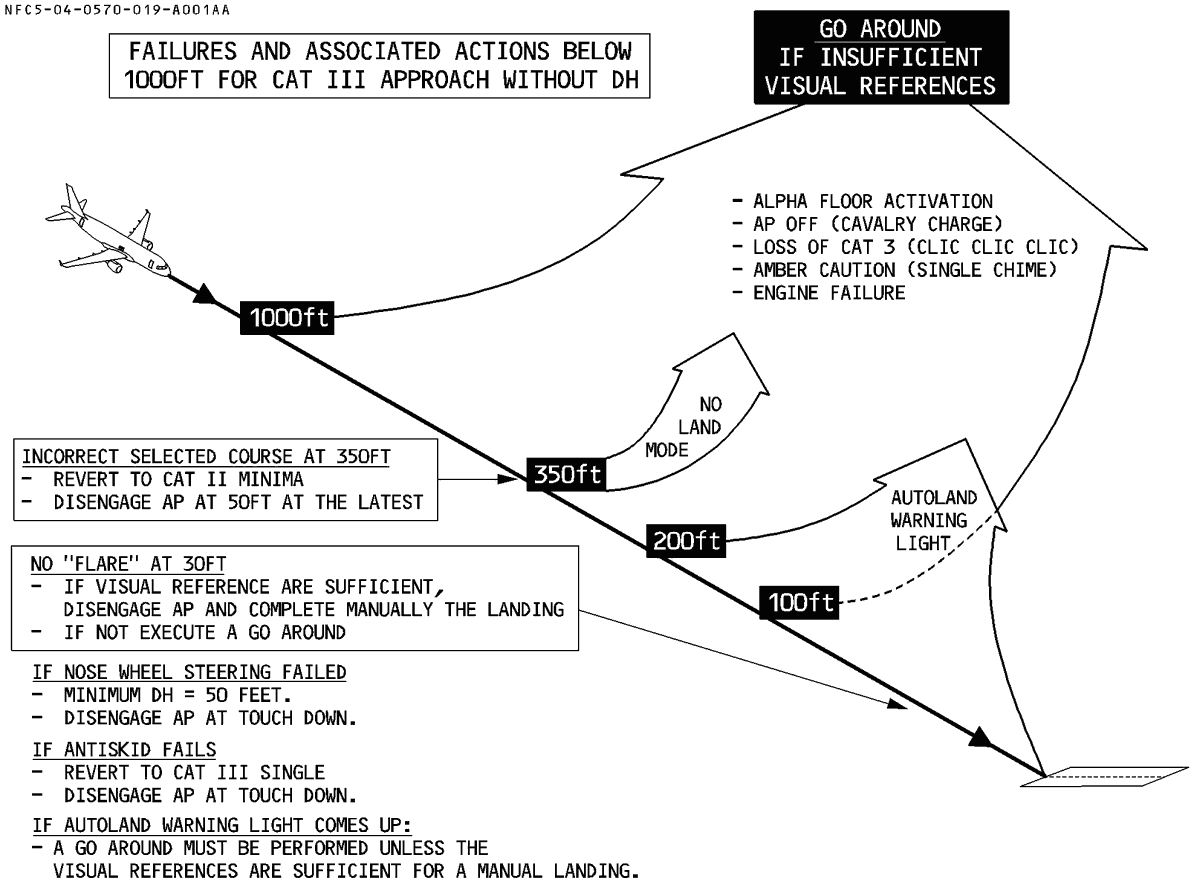
\includegraphics{images/catIII-failures.png}}}\vspace*{\fill}

\end{document}
